\chapter{Introduction\label{chap:introduction}}

\section{Small molecule drug design\label{sec:drug-design}}
The discovery of novel drugs has contributed significantly to the improvement of human health and
well-being. There is continous demand for new drugs, in order to expand the range of treatable
diseases, to improve the efficacy of existing treatments and to respond to the emergence of new
diseases.

Small molecule drugs are the major kind of medicines in use, constituting as much as 90\% of global
sales \citep{makurvetBiologicsVsSmall2021}. Small molecules are usually defined as molecules with a
molecular weight of less than 900 Da. These molecules are usually orally available, have good
pharmacokinetic properties and can be synthesized in a cost-effective manner.

For a small molecule to be a viable drug candidate it needs to fulfill a whole range of properties \citep{todo}:
\begin{itemize}
      \item \textbf{On-target activity:} The molecule needs to be active against the desired target in
            order for it to show the desired therapeutic effect. On a molecular level this means that the
            molecule needs to bind to the target and modulate its activity in the desired way.
      \item \textbf{Pharmacokinetics:} The molecule must have favourable pharmacokinetic properties
            such as adsorption, distribution, metabolism and excretion (ADME). ADME determine how the
            molecule is absorbed into the body, how it is distributed in the body, how it is metabolized and
            how it is excreted from the body. These properties are crucial for the molecule to reach the
            target in the body and to be metabolized in a safe manner and to finally be excreted from the
            body.
      \item \textbf{Toxicity:}  The absence of toxic effects is crucial, as the molecule must be
            well-tolerated and devoid of any potential harmful side effects. Toxicity can be caused by a
            range of factors, including off-target interactions, metabolic byproducts or allergies.
      \item \textbf{Specificity:}  The molecule should exhibit high specificity, selectively
            interacting with the intended target while minimizing undesirable off-target interactions.
            Off-target binding can lead to adverse side effects and potentially compromise the drug's safety
            and efficacy profile.
      \item \textbf{Synthesis:} The molecule must be synthesizable in a cost-effective manner to be
            practically useful.
      \item \textbf{Patentability:} The molecule must be novel and not infringe on any existing
            patents. While in general this is not needed for a drug to work, this constitutes a significant
            issue in practice.
\end{itemize}

The main challenge in drug discovery is to find a molecule that fulfills all these mentioned
properties. The development of a new drug is a complex and expensive process, which can take up to
10-15 years and costs up to 3 billion USD \citep{todo}.


\subsection{The drug discovery pipeline}
The drug discovery process is usually divided into several stages depicted in \Cref{fig:drug-discovery-pipeline} and described below.

\begin{figure}
      \centering
      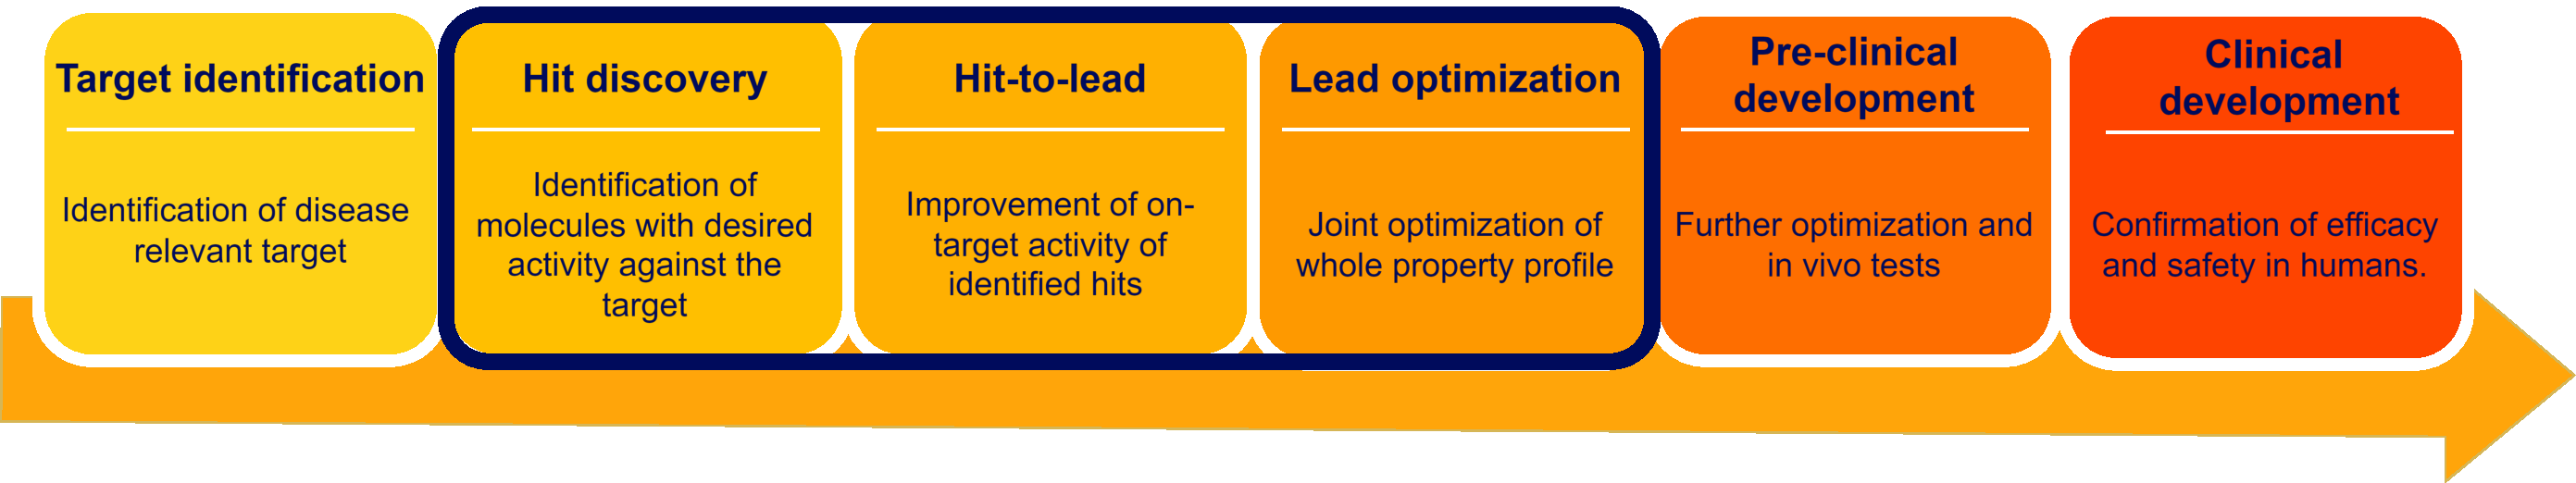
\includegraphics[width=\textwidth]{figures/drug-discovery-pipeline.pdf}
      \caption{The drug discovery pipeline starts with the identification of a biological target. Once
            a target is identified, readily available molecules are screened for their activity against the
            target in high-throughput screening. Promising hits are then modified and optimized to lead
            compounds. These lead compounds are then further optimized and tested in preclinical. Finally,
            the most promising candidates are tested in clinical trials and eventually approved by
            regulatory agencies. The stages in the blue box are highly amenable to machine learning and
            computational methods and are the focus of this thesis. \label{fig:drug-discovery-pipeline}}
\end{figure}
\begin{itemize}
      \item \textbf{Target identification:} The drug discovery process starts with the identification
            of a biological target, which is a molecule or a protein that is involved in a disease
            process.
      \item \textbf{Hit discovery:} In the hit discovery stage molecules are screened for their
            activity against the target in high-throughput screening (HTS). These lab experiments, often
            referred to as assays, are used to measure the activity of the molecules against the target in
            vitro. This stage results in a set of so called hits, which are molecules that show activity
            against the target.
      \item \textbf{Hit-to-lead:} Promising hits are then modified and optimized to lead compounds. In
            this stage, the optimization is primarily focused on improving the activity of the molecule
            against the target. This is usually done in a DMTA (Design-Make-Test-Analyze) cycle, where the
            molecule is designed, synthesized, tested in vitro. The results are then analyzed and the cycle
            continues until a satisfactory lead compound is found.
      \item \textbf{Lead optimization:} The lead compounds are then further optimized to improve their
            properties, such as pharmacokinetics, toxicity or specificity. This is usually done in a DMTA
            cycle as in the hit-to-lead stage and also involves the synthesis and testing of the molecules
            in vitro.
      \item \textbf{Preclinical development:} The most promising candidates are then tested in
            preclinical studies. These studies are usually done in animals and are used to assess the safety
            and efficacy of the drug candidate in vivo.
      \item \textbf{Clinical trials:} Finally, the candidates that pass the preclinical studies are
            tested in humans in clinical trials. These are usually divided into three phases, where the
            safety and efficacy of the drug are tested in increasing numbers of patients. Phase I trials are
            mainly focused on the safety of the drug, Phase II trials are focused on the efficacy of the
            drug and Phase III trials are focused on the safety and efficacy of the drug in a larger
            population.
      \item \textbf{Regulatory approval:} The final stage is the regulatory approval, where the drug
            is approved by regulatory agencies such as the FDA in the US or the EMA in Europe.
\end{itemize}

The general strategy of this stagewise approach is to reduce the uncertainty about the usefulness of
a molecule at each stage. The earlier stages are usually cheaper and faster, but have higher
uncertainty about the clinical success of the molecule. The later stages are more expensive and
slower, but provide better information about the success chances of a molecule.

The success rates of clinical trials are low, with only about 10\% of drugs that enter clinical
trials eventually being approved by regulatory agencies More specifically, the success rates in
Phase I/II/III and the final regulatory approval are 63\%, 31\%, 58\% and 85\% respectively
\citep{mullardParsingClinicalSuccess2016}. This translates to 63\%, 19.5\%, 11.3\% and 9.6\% of
projects that make it to the respective stages \citep{mullardParsingClinicalSuccess2016}.

\subsection{The Design-Make-Test-Analyze cycle}
\begin{figure}
      \centering
      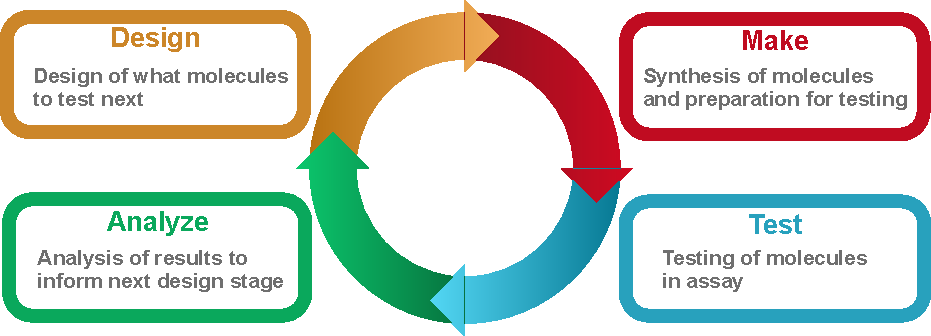
\includegraphics[width=\textwidth]{figures/dmta_cycle.pdf}
      \caption{The DMTA cycle}
\end{figure}
The hit discovery, hit-to-lead and lead optimization stages (blue box in
\Cref{fig:drug-discovery-pipeline}) usually operate in an iterative manner, resulting in a cycle of
choosing molecules to be tested, synthesizing them, testing them in laboratory experiments and analyzing the
results to guide the selection of the next molecule to be tested. This cycle is usually referred to as the
\ac{DMTA}-cycle:
\begin{itemize}
      \item \textbf{Design:} Under consideration of previous experimental results, the molecule(s) to be tested
            are designed. The design generally aims to optimize the desired properties of the molecule, but
            also aims to maximize the information gained from the experiment. This stage often relies on
            computational methods to predict the properties of the molecules.
      \item \textbf{Make:} The designed molecules are then synthesized in the laboratory. This step requires
            a synthesis plan that outlines the steps needed to synthesize the molecule.
      \item \textbf{Test:} The synthesized molecules are then tested in laboratory experiments to
            measure the properties of interest.
      \item \textbf{Analyze:} The results of the experiments are then analyzed.
            involves the evaluation of the performance of the prediction models used in the design
            phase. The results of the analysis are then used to guide the design of the next molecule
            to be tested.
\end{itemize}

Computational methods are widely used throughout the DMTA cycle.
One of the most important applications of computational methods in drug discovery is the prediction of
the properties of molecules. These properties can range from the activity of a molecule against a
target, to its pharmacokinetic properties, to its toxicity. These \ac{QSPR} models are used to
predict the properties of molecules in the design phase, to guide the selection of molecules to be
tested.

In recent years there has been increased interest in the use of generative models to solve various
tasks in drug discovery. These models can be employed for more complex tasks that require the
model outputs to be molecules. In this thesis we focus on two application areas, de novo drug design
and computer-aided synthesis planning, which we will introduce in the following sections.

\subsection{De novo drug design}
\Ac{DNDD} \citep{schneiderNovoMolecularDesign2013} is a computational approach for automatically designing molecules with desired property
profiles. \Ac{DNDD} expands upon \ac{VS}, a method in which a library of molecules is ranked
according to the output of a \ac{QSPR} model. \citet{waltersVirtualChemicalLibraries2019} estimates
that approximately $10^{13}$ molecules can be routinely tested in a \ac{VS} experiment. While this
number can vary significantly depending on the computational cost of running the \ac{QSPR} model, it
is dwarfed by the size of drug-like chemical space, which is estimated to contain between $10^{30}$
and $10^{60}$ molecules
\citep{waltersVirtualChemicalLibraries2019,ruddigkeitEnumeration166Billion2012}. Consequently,
\ac{VS} is limited to exploring only a small fraction of chemical space and cannot fully leverage
the vast possibilities that the entire chemical space offers.

% How does DNDD help
\Ac{DNDD} aims to address the limitations of \ac{VS} by focusing the search on the most relevant
parts of chemical space. In contrast to the static library approach of \ac{VS}, de novo design
proceeds in an iterative fashion, exploring chemical space in a goal-directed manner. This iterative
process addresses the efficiency problem of virtual screening by dynamically concentrating the
search on promising molecules. As the algorithm progresses, it learns from previous iterations,
refining its search strategy and potentially discovering novel molecular structures that may not be
present in predefined libraries.

% Recent hype
Recently, the field of de novo drug design has seen a surge in interest, as advances in deep learning
have triggered the development of many new deep learning-based generative models for de novo drug
design \citep{eltonDeepLearningMolecular2019}. A multitude of different models have been proposed,
which are based on a variety of neural network architectures, training strategies and molecular
representations \citep{eltonDeepLearningMolecular2019,sanchez-lengelingInverseMolecularDesign2018}.
These models have shown great promise in generating novel molecules with desired property profiles
and have been used in a variety of applications, such as the design of new drugs, materials or
catalysts \citep{todo}.

%Evaluation of generative models
However, the evaluation of \ac{DNDD} models, and generative models in general, is more challenging
than the evaluation of discriminative models. While the performance of discriminative models can be
evaluated on a hold-out test set, \ac{DNDD} methods aim at generating novel molecules. By definition
of the task, there is no ground truth set of molecules to be discovered. While models
can in principle be evaluated by the scores of the generated molecules, this one-dimensional
evaluation is often insufficient to capture the performance of the model in practical settings.
While there has been work on developing better evaluation metrics and benchmarks
\citep{brownGuacaMolBenchmarkingModels2019,polykovskiyMolecularSetsMOSES2020,thomasComparisonStructureLigandbased2021,gaoSampleEfficiencyMatters2022,trippFreshLookNovo}
the evaluation of generative models is still an active area of research and challenges remain.

\begin{figure}
      \centering
      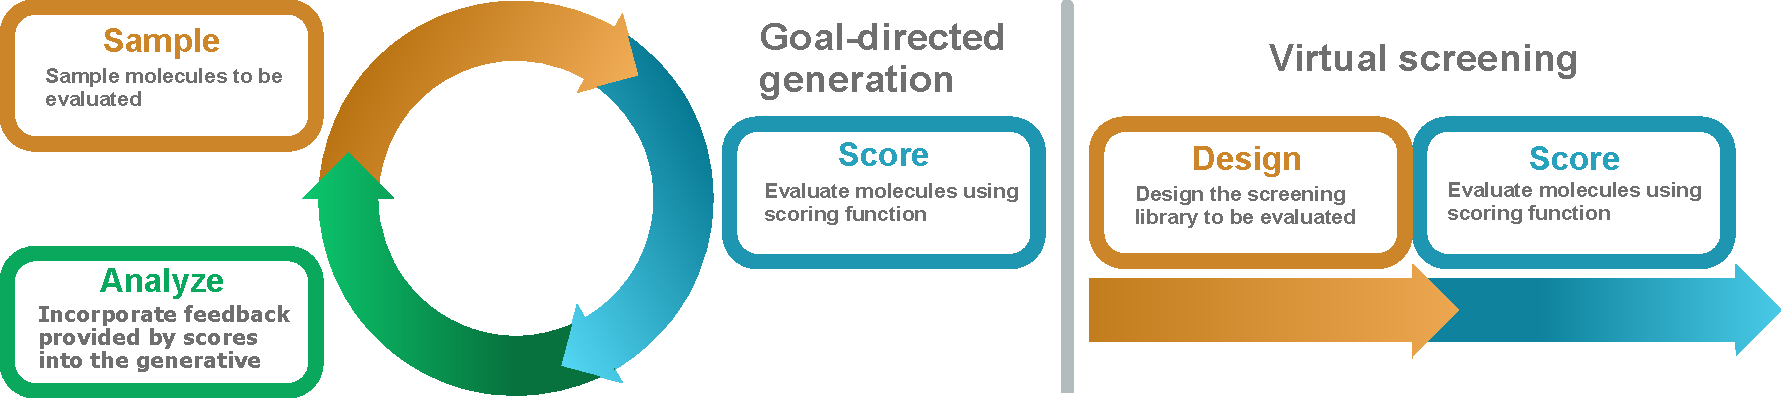
\includegraphics[width=\textwidth]{./figures/goal_directed_cycle_and_virtual_screening.pdf}
      \caption{Comparison of goal-directed generative models and virtual screening. Goal-directed
            generation proceeds in a loop where already scored molecules inform what molecules to test next.
            Virtual screening proceeds in a linear fashion, where the molecules to be tested are determined
            beforehand. }
\end{figure}

\subsection{Computer-aided synthesis planning}
Drug candidates, whether suggested by generative models or found by other means, at some point need
to be synthesized in for further testing and eventually for use in patients. The synthesis of a
molecule is usually a complex process, involving multiple steps of chemical reactions.
Computer-aided synthesis planning (CASP) can help by finding new synthesis routes for a target
molecule. In some cases, this can lead to more efficient and cheaper synthesis routes, or even
enables the synthesis of previously inaccessible molecules.

% Synthesis planning 
The most popular approach to CASP is retrosynthesis planning. Starting from a target molecule, the
goal is to predict a chain of chemical reactions that can transform readily available starting
materials into the target molecule. This problem is usually formulated as a graph search problem,
where the nodes are molecules and the edges are chemical reactions. The goal is to find a path from
the target molecule to a set of starting materials, which can be synthesized in the laboratory. The
connectivity of this graph is given by retrosynthesis prediction models, which given a target
product, predict which reactants it can be made from. Highly accurate retrosynthesis prediction
models are necessary for the success of CASP tools, as otherwise the suggested synthesis routes
might not be feasible in the laboratory.

% A prominent approach to CASP is template-based planning Mention transformers and graph-based
% models
Template-based models are a popular approach to retrosynthesis prediction. These models use so
called reaction templates, which are graph transformation rules that encode connectivity changes
between atoms during a chemical reaction. These templates can be either automatically extracted from
a reaction database or hand-coded by a chemist. Given a target molecule, the goal is then reframed
as a classification task, where the model predicts which templates can be used to synthesize the
target. Application of the graph transformation rules then leads to reactants that can be used to
synthesize the target molecule. While popular, these models have some limitations, in common
datasets many templates only occur in few training samples, which makes it difficult to train a
model that generalizes well for these rare templates.

\newpage
\section{Generative Models in Drug Discovery\label{sec:generative-models}}
Triggered by advances in deep learning, the field of generative models for molecules has seen a
surge in interest in recent years. The first deep-learning based generative models for molecules
were based on recurrent neural networks (RNNs) originally proposed for text generation. After this
early work by \citep{seglerGeneratingFocusedMolecule2018} and
\citep{gomez-bombarelliAutomaticChemicalDesign2018} a great number of different models have been
published \citep{eltonDeepLearningMolecular2019,sanchez-lengelingInverseMolecularDesign2018}. These
models are based on a large variety of architectures and training strategies, including
autoregressive models, generative adversarial networks (GANs), variational autoencoders (VAEs),
flow-based models \citep{madhawaGraphNVPInvertibleFlow2019}. One key design choice is the
representation of the molecules, which can be based on SMILES strings, graph-based representations
or 3D structures
\citep{eltonDeepLearningMolecular2019,sanchez-lengelingInverseMolecularDesign2018,pangDeepGenerativeModels2024}.

% Generative model introduction 
Generative models are a class of machine learning models that generate new data samples. This is in
contrast to classification/regression models, which predict a label or a continuous value for a
given input. In the context of small molecule drug design, generative models are used to generate
molecular structures that are relevant to a given task. These tasks can range from de novo design, to linker optimization,
and to reaction prediction.

In this section we give a short overview of different generative models. We start with different
ways to represent molecules and then discuss different approaches to generate molecules. We will
then give an overview of three important generative modelling tasks in drug discovery: de novo drug
design and computer-aided synthesis planning.



\subsection{Molecular Representations}
\begin{figure}
      \centering
      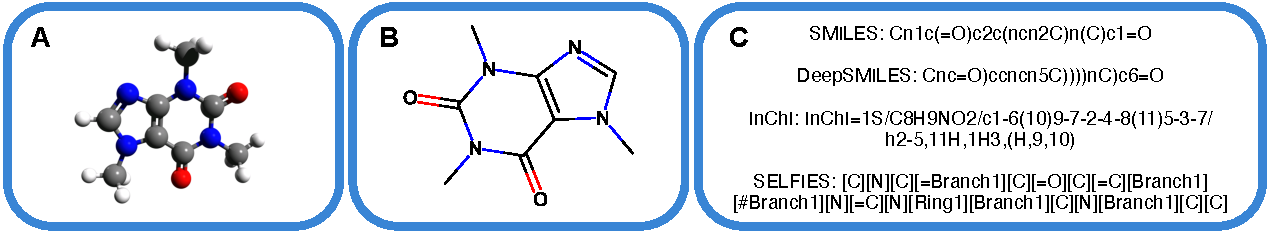
\includegraphics[width=\textwidth]{figures/representations/representations.pdf}
      \caption{Different ways to represent molecules. The molecule shown is caffeine \textbf{A:}
            Different 1D representations of a molecule. SMILES is an established line notation for
            molecules. DeepSmiles enables easier generation of molecules by getting rid of pair brackets and
            ring numbers. SELFIES guarantees that a sequence of tokens parses into a valid molecule.
            \textbf{B:} 2D graph representation of a molecule. The nodes represent atoms and the edges
            represent bonds. \textbf{C:} 3D structure of a molecule. The atoms are positioned in 3D space.
            The positions of these atoms can change as some bonds are allow rotations. Source of the 3D
            structure: \citep{EnglishCaffeine3D2010}. \label{fig:molecular-graph}}
      % TODO: add adjacency matrix representation
\end{figure}
Molecules are complex objects that can be represented in a variety of ways. While molecules are
complex quantum mechanical objects, there exist a variety of more simple, practically useful
representations of molecules. Molecules are formed by atoms, which are connected by chemical bonds.
The connectivity between the atoms can be represented as a graph, where the nodes represent atoms
and the edges represent bonds. In addition to the connectivity, atoms and bonds have other
properties, such as their type, charge or chirality. These properties are represented as node or
edge features in the graph. The graph structure of a stable molecule does not change and defines
the molecule's identity.

Molecules can also be represented as a 3D structure, where the atoms are positioned in 3D space.
This representation is useful for studying the interactions of molecules with other molecules or
proteins.

Molecular graphs can also be linearized into a 1D sequence of characters. Line notations such as
INCHI \citep{todo} or Simplified Molecular Input Line Entry System (SMILES)
\citep{weiningerSMILESChemicalLanguage1988} represent molecules as 1D representations of characters.
SMILES strings have turned out to be a highly useful representation of molecules in the context of
generative models, as they are easily processed by sequence-based models such as recurrent neural
networks (RNNs) or transformers \citep{vaswaniAttentionAllYou2017}. Several extensions for this
molecular representation have been proposed, such as SELFIES
\citep{krennSELFIESFutureMolecular2022}, DeepSmiles \citep{oboyleDeepSMILESAdaptationSMILES2018} or
SAFE \citep{noutahiGottaBeSAFE2023}.

\subsection{Generative modelling approaches}
There is a wide variety of approaches to generate molecules. The main differences between approaches
relate to molecular representation, the used training objective and the way molecules are sampled.
In the following section, we will provide an overview of several widely-adopted approaches to
molecular generation.

\subsubsection{Rule-based models}
% https://www.frontiersin.org/journals/hematology/articles/10.3389/frhem.2024.1305741/full#h4
Rule-based models generate molecules by applyng a set of pre-defined graph transformation rules to
combine molecular fragments. These rules are often manually defined. A popular approach is to
transformations that represent chemical reactions, as this encourages the generation of
synthesizable molecules. Those rules can either transformations that represent chemical reactions.
Notable examples of this approach are:
\begin{itemize}
      \item Fragment spaces: The BRICS \citep{degenArtCompilingUsing2008} method provides a set of
            molecular fragments and rules how to meaningfully combine them. This enables the generation of
            new molecules by combining these fragments.
      \item DOGS \citep{hartenfellerDOGSReactionDrivenNovo2012} provides a set of readily available
            building blocks and synthetic principles how to combine them.
            % TODO: MOVE \item
            % \citep{bradshawBarkingRightTree2020,gottipatiLearningNavigateSynthetically2020} formulates a
            % general framework of creating synthesis graphs relying on a chemical reaction model.
      \item \citep{jensenGraphbasedGeneticAlgorithm2019} defines graph mutation and crossover
            operations to generate new molecules.
\end{itemize}
These models allow the generation of molecules that are chemically valid, or resemble known
"reasonable" molecules. While basic properties of the generated molecules can be made to resemble a
training set, these models do not allow more complex training objectives.

\subsubsection{Autoregressive string-based models}
Autoregressive string-based models constitute one of the most popular approaches to generative
models for generating discrete 1D/2D molecular representations. These models start with an "empty"
molecule and iteratively add to it. At each step, the model takes the current state of the molecule
chooses a modification to apply from a set of possible modifications. This modification is then
applied to the molecule and the process is repeated until a special end-of-sequence action is taken.
Mathematically this can be formulated as
\begin{align}
      p(x) = \prod_{i=0}^n p(x_i | x_{1:i-1}),
\end{align}
where $x$ is the molecule and $x_i$ corresponds to the state of the molecule at step $i$. This gives
us a probability distribution over the space of molecules and to evaluate the likelihood of a given
molecule. Models for which this fact holds are called explicit density models.

One of the most popular approaches is to use recurrent neural networks (RNNs) or Transformer models
\citep{vaswaniAttentionAllYou2017} model 1D sequences. These models have been used to generate
SMILES, SELFIES or DeepSmiles strings \citep{seglerGeneratingFocusedMolecule2018,todo}. In most
cases, the training data is a set of molecules and the model is trained to maximize the likelihood
of the training data. The molecules are usually tokenized into the grammatical units of the used
representation before training. The model is then trained to predict the next token in the sequence
given the previous tokens.

Another approach to autoregressive modelling is to use graph-based models, which model the molecular
graph directly. These models are based on graph neural networks (GNNs) and are used to generate
molecular graphs directly. These models start with an empty graph and iteratively add nodes and
edges to it. At each step the model chooses a modification to apply to the graph and applies it.
While the specification of possible actions is usually more complex than in the 1D case, the model
can be trained in a similar manner.

\subsubsection{Graph-based autoregressive models}
\subsubsection{Variational autoencoders}
\Acp{VAE} are another popular approach to generate molecules. \Acp{VAE} are latent space models,
which sample data by first sampling from a simple latent distribution $p(z)$, which is often a
multi-variate normal distribution. The samples are then mapped to molecular space via a
probabilistic decoder network $p(x|z)$. To make training tractable a second network, the encoder
network $q(z|x)$ is used to map the data to the latent space. The model is trained to maximize the
evidence lower bound (ELBO) of the data
\begin{align}
      \log p(x) \geq \mathbb{E}_{q(z|x)}[\log p(x|z)] - \text{KL}(q(z|x) || p(z)),
\end{align}
where KL is the Kullback-Leibler divergence. This model has the advantage of providing a continuous
latent space, which can be used to interpolate between molecules and allows to run continuous
optimization algorithms in latent space. The exact likelihood of a given molecule cannot be
calculated exactly as integration over the latent space
\begin{align}
      p(x) = \int p(x|z) p(z) dz,
\end{align}
is not tractable. However, the likelihood can be approximated by sampling latent states $z_i ~
      q(z|x)$ and averaging over the likelihood of the data given the latent state $p(x|z_i)$.

\subsubsection{GFlowNets} ...

% molgan
\subsubsection{Generative adversarial networks}
\Acp{GAN} are similar to VAEs in that they also sample from a simple distribution in latent space,
$p(z)$ and map the samples to molecular space via a generator network $p(x|z)$. However, the
training of GANs is based on a game-theoretic approach, where a generator network is trained to
generate samples that are indistinguishable from the training data. The training signal is provided
by a discriminator network, which is trained to distinguish between real and generated samples. The
generator is then trained to minimize the discriminator's ability to distinguish between real and
generated samples. GANs have been used to generate molecules in a variety of representations
\citep{todo}. In general the generator network is not invertible, which means that the likelihood of
a given molecule cannot be calculated. This makes GANs implicit density models, which define a
likelihood function $p(x)$ only implicitly via sampling, but not explicitly.

\subsubsection{Generative flows}
% moflow, graphnvp (has nice discussion on one-shot generation)
Generative flows are based on the idea of learning a bijective`' mapping between the data space and
a latent space. These models sample molecules by first sampling from a simple distribution in latent
space, $p(z)$ and then mapping the samples to molecular space via a bijective mapping $G: z
      \rightarrow x$. The model is trained to maximize the likelihood of the training data, which can be
calculated exactly via the change of variables formula:
\begin{align}
      p(x) = p(z) \left| \det \frac{\partial G}{\partial z} \right|.
\end{align}
The mapping $G$ is usually implemented as a neural network, which consists of a series of invertible
transformations, which combined can approximate complex transformations. These models were first
introduced for continuous data \citet{rezendeVariationalInferenceNormalizing2016}. The extension to
molecules, which are discrete data, necessitates using a continuous relaxation of the molecule. This
is often done by modelling the adjacency/node feature matrix of the molecule as a continuous
variable. These models also belong to the class of explicit density models, as the likelihood of a
given molecule can be calculated exactly.

\subsection{Auto-encoders}
\citep{polykovskiyEntangledConditionalAdversarial2018,winterLearningContinuousDatadriven2019}

\paragraph{Diffusion models} also rely an a variational bound and are approximate density models.

\paragraph{Alternative approaches} There are a variety of alternative approaches such as 3d
modelling which we will not discuss in detail here.



\subsection{Distribution-learning}
One core application of generative models is to learn to sample molecules that resemble the training
data in distribution. The core idea is to learn what stable molecular structures look like, much
like a language model learns how to generate coherent text. Such a model can then serve as a base
for other applications, such as goal-directed generation, which we will discuss in the next section.

Assuming the true distribution of molecules is $p(x)$, the goal of a distribution-learning model is
to learn a model $q(x)$ that approximates the true distribution as closely as possible. This can be
done by minimizing the cross-entropy between the true distribution and the model distribution
\begin{align}
      \mathcal{L} = - \mathbb{E}_{x \sim p(x)} \log q(x).
\end{align}
Molecules are then sampled from the model distribution $q(x)$.

Methods suitable for distribution-learning include all explicit, approximate and implicit density
models. Those models and their respective training strategies learn to approximate the distribution
of a given training set of molecules. However, one can also use rule-based models such as
\citep{jensenGraphbasedGeneticAlgorithm2019}, which are not based on a learned model of the data
distribution, but rather on a set of rules that define the distribution of molecules.

% Generative models are often divided into two categories: \emph{goal-directed} and
% \emph{distribution-learning} models. Distribution-learning models learn general structural
% patterns in molecules and aim to sample novel molecules that resemble the training data in
% distribution. These models are then most often used as a base for goal-directed models, which aim
% to find molecules that satisfy a property profile of interest. These properties are usually
% encoded in a scoring function, which is then used to guide the generation process, in a
% reinforcement learning style feedback loop.

% % The evaluation of generative models is challenging. While generative models have shown great
% promise in generating stable chemical structures their evaluation is often challenging. While
% evaluation in discriminative tasks is usually a straightforward evaluation on a hold-out test set,
% the evaluation of generative models requires more complex evaluation schemes and require to take
% into account various aspects of the generated molecules. This has led to the development of a
% range of evaluation metrics
% \citep{preuerFrechetChemNetDistance2018,gaoSynthesizabilityMoleculesProposed2020} and benchmarks
% for generative models
% \citep{polykovskiyMolecularSetsMOSES2020,brownGuacaMolBenchmarkingModels2019}. However, the
% evaluation of generative models is still an active area of research and challenges remain. In this
% thesis, we address some of these challenges which are outlined in the following sections.

\subsubsection{Evaluation of distribution-learning models}
The evaluation of distribution-learning models can be challenging. While the performance of
explicit/approximate density models can be evaluated and compared using the \ac{NLL} and related
metrics like the perplexity, implicit density models do not offer a straightforward evaluation.
Generative adversarial networks (GANs) \citep{goodfellowGenerativeAdversarialNetworks2014} do not
offer the possibility of this a straightforward evaluation. To this end alternative metrics have
been proposed, spawning its own subfield of research \citep{heuselGANsTrainedTwo2017}.

In the field of cheminformatics new metrics have been proposed to evaluate the quality of generated
molecules and how well they match the training data in distribution. Among these are the FCD metric
\citep{preuerFrechetChemNetDistance2018}, the internal diversity
\citep{benhendaChemGANChallengeDrug2017} of the generated molecules, or the KL-divergence between
the distributions of chemico-physical properties of the generated molecules and the training data.
The Moses \citet{polykovskiyMolecularSetsMOSES2020} and GuacaMol
\citet{brownGuacaMolBenchmarkingModels2019} aim to provide a standardized benchmark for generative
models. However, those evaluations use ad-hoc metrics that are not necessarily informative about
actual model performance.

\subsection{Goal-directed generative models\label{sec:eval-gen}}
\subsubsection{Optimization strategies}
% General desciption
Goal-directed generative models\footnote{This is a bit of a misnomer as of course all generative
      models pursue a goal. However, in general the term is used to include only models that aim at
      optimizing a given scoring function. } are tasked with finding molecules maximize a given property
profile. This property profiles is encoded by a \ac{QSPR} model which assign a score, $s(x)$, to
each molecule $x$. The goal of the generative model is then to find molecules that maximize the
score. This can be done by sampling molecules from the model distribution, evaluating the score of
the molecules and then updating the model distribution to increase the probability of sampling high
scoring molecules.

% How does it compare to VS
Virtual screening is an alternative approach that instead of generating molecules specifically for a
given task, evaluates molecules from a fixed library. This has advantages in that the molecules can
be selected from synthetically accessible libraries, but has the disadvantage that the search is not
guided by the feedback of already tested molecules.

% How is it done?
There are different ways to implement this feedback loop:
\begin{itemize}
      \item \textbf{Hill-climbing} is a simple optimization algorithm that relies on a
            distribution-learning model. Molecules are sampled from the model distribution, their scores are
            evaluated and then the model is retrained on the high-scoring molecules. This process is
            repeated until a stopping criterion is met.
            % mars segler
      \item \textbf{Reinforcement learning} uses the molecule scores as a reward signal to update the
            model distribution. This is most often done via the REINFORCE algorithm
            \citep{williamsSimpleStatisticalGradientfollowing1992}.
      \item \textbf{Genetic algorithms} transform an initial population of molecules by applying
            mutations and crossovers. The molecules are then evaluated and the best ones are selected for
            the next generation. Applying this process iteratively leads to a population of high-scoring
            molecules.
      \item \textbf{Tree search}: ??
\end{itemize}


\subsubsection{Exploitation of scoring functions}
% Overfitting to the scoring function
When training goal-directed generative models, it is important to be aware of the limitations of the
scoring function. This is especially important in the when using \ac{ML} based scoring functions.
This is because goal-directed generators try to find an input that maximizes the output of the
\ac{ML} model. It is well known that this strategy can fail miserably, as the generative model can
optimize the output of the \ac{ML} model in ways that are not actually relevant. In the image
domain, this was found to lead to samples that are obviously misclassified and in the most extreme
case to adversarial examples \citep{todo}. % brittle, adversarial

Another problem in this setting is that \ac{ML} models can show biases towards the training samples.
This is because models usually usually show much better performance on the training data than on new
data. This can give the generative model an incentive to generate samples that are similar to the
training data, which can lead to a lack of novelty in the generated molecules.

It is currently unclear whether this is a problem in the context of generative models for molecules.
However, it is likely that the generative models can overfit to irrelevant features that do not
actually contribute to the desired properties of the molecules.

\subsubsection{Diversity}
The diversity of the generated molecules is an important aspect in the application of goal-directed
generative models. Given that the scoring functions are usually only an imperfect and incomplete
approximation of the desired properties, finding a diverse set of molecules that score well can
increase the success chancess of downstream stages of the drug discovery project. Given the expected
failure of some of the candidates in later experiments, having a backup of other candidates with
somewhat different structure can be beneficial.

It is unclear how well current generative models perform in generating diverse high-scoring
molecules, which is due to a combination of two main factors. Firstly, many commonly used diversity
metrics are inadequate for evaluating diverse optimization approaches. This results in uninformative
benchmarks that do not meaningfully measure the diversity of the generated molecules. Secondly, a
meaningful comparison of goal-directed generators necessitates a standardized compute budget. This
is because the performance of generative models depends strongly on the amount of ressources
available for training and evaluation.

\subsubsection{Standardized compute budgets}
Another challenge in the evaluation of goal directed models is the lack of standardized compute
budgets. Fundamentally optimizing molecular properties is a search problem that - given infinite
ressources - can be solved by brute force enumeration of chemical space. Thus the main challenge of
de novo design is to arrive at high scoring molecules with a limited amount of ressources, which is
in fact often given as the main reason to use goal-directed models in the first place \citep{todo}.
Therefore, a meaningful comparison of goal-directed models necessitates a standardized compute
budget.

However, in many studies different models are compared without taking this into account. Therefore,
it might well be the case that some algorithms are run for days or weeks, while others are only run
for minutes or hours. The latter might, however, be able to outperform the former if given the same
amount of ressources.

The computational cost of running an experiment depends on these main factors:
\begin{itemize}
      \item The cost of generating a molecule
      \item The cost of evaluating a molecule
      \item The sample efficiency of the optimization algorithms
\end{itemize}

The cost of generating a molecule depends on the generative model used. While more complex models,
e.g. deep learning models, are usually more computationally expensive, simpler models can be run
with less ressources. The cost of calculating the score of a molecule depends on the scoring
function used. The used scoring functions can be anything from simple physico-chemical properties,
to more complex machine learning models. Docking simulations are usually even more expensive and in
the extreme case one could directly optimize the results of in vitro experiments. The sample
efficiency measures how many molecules need to be generated and evaluated in order to find good
solutions.

There is an interesting interplay between the importances of these three factors. The sample
efficiency gets more important the more expensive molecule generation and evaluation are. For
expensive scoring functions like docking simulations, the generation cost with current models can
often be neglected and the sample efficiency is becomes the sole factor determining the performance
of an algorithm. For cheap scoring functions like physico-chemical properties, or less complex
machine learning models, and the performance of the algorithm depends on a combination of the
generation cost and the sample efficiency.

\subsection{Retrosynthesis Prediction\label{sec:retrosynthesis}}
\subsubsection{Modelling approaches}
% Retrosynthesis prediction is a popular application of generative models in drug discovery. Given a  


In \citep{seidlImprovingFewZeroShot2022} we study the problem of single-step retrosynthesis
prediction. Given a target molecule, the goal is to predict a set of reactants that can be used to
synthesize the target molecule. Template-based models are a popular approach to single-step
retrosynthesis prediction. These models use so called reaction templates, which are either extracted
from a reaction database or hand-coded by a chemist. Given a target molecule, the goal is then
reframed as a classification task, where the model predicts which templates can be used to
synthesize the target.



\section{Aims and Objectives\label{sec:aims-objectives}}
\subsection{Highlighting Failure Modes in Evaluating Generative Models}
In \citep{renzFailureModesMolecule2019} (\cref{sec:failure-modes}) we show the limitations of the
GuacaMol distribution-learning benchmark, by evaluating the performance of different sophisticated
generative models on this benchmark, and comparing it to a simple baseline model that generates
molecules by introducing minor variations of the molecules in the training data. We show that the
most of the tested generative models do not outperform the simple baseline model, or only do so
marginally. This suggests that the tested benchmarks are not be able to distinguish state-of-the-art
generative models from simple baseline models, and call for a more comprehensive evaluation of
distribution-learning models. \Cref{sec:failure-modes} reprints the corresponding publication.

In \citep{renzFailureModesMolecule2019} we introduce \emph{control scores} that give information
whether the optimization overfits to artifacts of the scoring functions, or the training data. We do
this by training additional scoring functions, trained with either a different random initialization
or trained on a hold-out subset of the the available training data. Using this approach, we can show
that generative models overfit to the scoring function's random initialization and to high-scoring
training samples. This shows that the reported performance of these models is an overestimation, and
that our control scores can be used to obtain a more meaningful evaluation of goal-directed molecule
generators. \Cref{sec:failure-modes} reprints the corresponding publication.

\subsection{Diversity-based benchmark of goal-directed generators\label{sec:divopt}} In
\citep{renzBenchmarkingEfficiencyGenerative2024} we introduce a benchmark for diverse optimization
that addresses the above-mentioned issues. In this benchmark, we evaluate the diversity of the
generated molecules using a recently proposed diversity metric \#Circles
\citep{xieHowMuchSpace2023}. We compare the performance of diverse optimization approaches under two
different compute budgets, namely a fixed number of scoring function evaluations and a fixed time
budget. The first setting is relevant for applications where the cost of evaluating the scoring
function dominates the optimization process, while the second setting is relevant for scoring
functions that are cheap to evaluate. Using this setup we test 14 goal-directed optimization methods
and show how SMILES-based auto-regressive models dominate the benchmark.
\Cref{sec:diverse-efficiency} reprints the corresponding publication.

\subsection{Improving few-shot and zero-shot retrosynthesis prediction}
In \citep{seidlImprovingFewZeroShot2022} we propose a novel approach to template-based
retrosynthesis prediction. We use a multimodal learning approach that learns to associate relevant
templates to product molecules using a Modern Hopfield Network
\citep{ramsauerHopfieldNetworksAll2020}. Our model can leverage structural information about the
templates and can make use of similarities between them. This allows for improved generalization,
especially for templates with few training samples and even for unseen templates. This model is
several times faster than comparable methods and shows good predictive performance.
\Cref{sec:mhn-react} reprints the corresponding publication.

\section{List of publications\label{sec:publications}} This thesis comprises the work published in
the following papers:

\begin{itemize}
      \item \fullcite{renzFailureModesMolecule2019}
      \item \fullcite{renzBenchmarkingEfficiencyGenerative2024}
      \item \fullcite{seidlImprovingFewZeroShot2022}
\end{itemize}

% give overview over my other publications
\paragraph{Other Publications} Besides the papers listed above, I have also contributed to the
following publications:

\begin{itemize}
      \item \fullcite{preuerFrechetChemNetDistance2018}
      \item \fullcite{renzUncertaintyEstimationMethods2019}
      \item \fullcite{hofmarcherLargescaleLigandbasedVirtual2020}
      \item \fullcite{renzLowCountTimeSeries2023}
\end{itemize}